\chapter{Design}
\label{chap:Design}

We aim to design stealthy \ac{SNI} and \ac{ALPN} encryption schemes based
on the basic premise that the 32 octets of the client and random
along with the 32 octets of the legacy session ID act as `cover',
which can be replaced with random-looking ciphertext.
There are other fields and extensions to the \ac{CH} message
which could provide additional cover,
but the \var{random} and \var{legacy\-\_session\-\_id}
provide cover of the highest quality; they are always present in a \ac{TLS} 1.3 \ac{CH},
their lengths do not vary between implementations, and they will not
need to be \ac{GREASE}'d.
In this dissertation
we focus our efforts on designs leveraging only these 64 octets of cover in the \ac{CH},
as well as the 32 octets of cover provided by the \ac{SH}\var{.random}.

\cite{rfc8744-issues} lay out a set of issues and design requirements pertaining to \ac{SNI} encryption, and the aim of this dissertation is design an \ac{SNI} encryption scheme that prioritises the requirement: ``Do Not Stick Out". However, a stealthy \ac{SNI} encryption scheme should of course also fulfill the other requirements listed by \cite{rfc8744-issues} where possible. Here we discuss these requirements and possible approaches to fulfilling them.

\section{Enable Multi-Party Security Contexts}
This requirements is about securely allowing the separation of the client-facing server and the backend server. In particular the protocol should protect the client from \ac{MITM} attacks. We can imagine a naïve design where a client-facing terminates the \ac{TLS} connection, the servername is indicated stealthily somehow, e.g. by prefixing it to the application data, and then the application is relayed to the backend server. In this design the client never authenticates the backend server, which means the client-facing server can act as a \ac{MITM} and delete, modify, reorder messages to/from the backend server without the client or backend server being able to detect these modifications.

\cite{rfc8744-issues} also point out that backend-server authentication is not sufficient,
and that the client-facing server should also be authenticated.
\ac{ECH} mitigates against \ac{MITM}
by having the client authenticate
the backend server using the regular
\ac{TLS} 1.3 mechanims,
but additionally there is an implicit authentication that the client-facing server owns the \var{ECHConfig},
i.e. it has the corresponding private key.
In order for the server
to produce the \ac{ECH} \var{accept\-\_confirmation} signal
it has to successfully decrypt the \ac{ECH} payload.
The cleartext of the payload is hard to 
guess because it contains a 32 octet random.

\ac{ECH} does not perform encryption of the secret \ac{SNI} parameter in the channel between
the client-facing and backend server,
which means this channel has to be protected
by some other means,
e.g. with a \ac{VPN} or a separate \ac{TLS} connection.

\cite{esni} distinguish two modes of operation for \ac{ECH}, shared mode and split mode.
In shared mode there is a single server which performs the \ac{ECH} decryption {\em and} terminates the \ac{TLS} connection,
whereas in split mode there is a client-facing server that performs \ac{ECH} decryption and which proxies the remaining \ac{TLS} traffic to and from a backend server which terminates the \ac{TLS} connection.
For \ac{ECH} each server is `aware' of its role in the ongoing connection.
The server can have a different role for different connections,
but within the context of a single connection the server determines its role based on the \var{type} field of the received \var{encrypted\_client\_hello} extension,
if the \var{type} is outer then the server is the client-facing server,
if it is \var{inner} the server is the backend server.

Figure~\ref{fig:sech-split-mode-accept} shows sequence diagram depicting the flow of messages in split-mode.

\begin{figure}[htb]
\centering
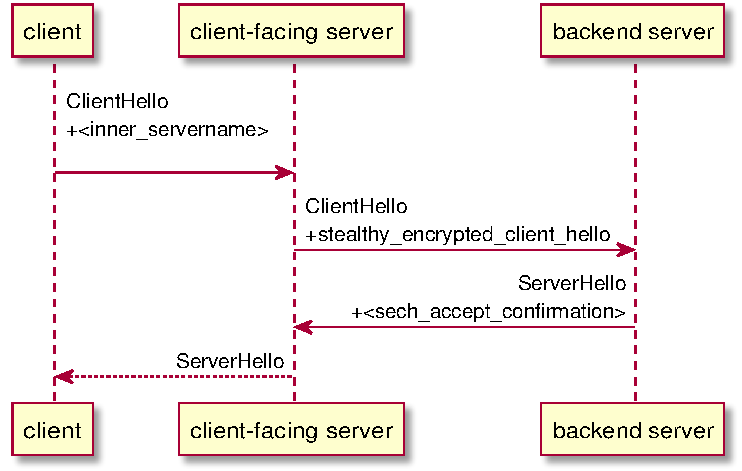
\includegraphics[width=\linewidth]{figure/sech-split-mode-accept.pdf}
\captionsetup{width=.8\linewidth} 
\caption[]{Sequence diagram for a successful SECH split-mode handshake.}
\label{fig:sech-split-mode-accept}
\end{figure}

For \ac{SECH} we don't have the luxury of setting
a cleartext \var{type} field to help the server
distinguish its role.
The approach we'll adopt below is to set the \ac{SNI} extension value in the \ac{CHI} to all 0s
as a signal that the server should act as a backend server.
The true \ac{SNI} is encoded elsewhere in the \ac{CH}.

The motivations for split-mode are:
1. to distribute workload,
and 2. to enhance privacy for the backend server and the user
(the client-facing server can't see application traffic).

One reason for hesitance in deploying split-mode may be that there's low incentive for large providers.
The provider loses access to application traffic,
which means it can't implement a \ac{WAF}.
Secondly the deployment and maintenance
of split-mode is more complex.

In this work we have aimed to provide a design that can facilitate a secure split-mode,
but we have not attempted to implement a
split-mode deployment.

\section{Active Attacks}

\label{sec:active-attacks}
Throughout the development of \ac{ECH} various
active attacks that might allow an attacker to discover inner \ac{CH} data
have been described and discussed.
In this section we describe how those attacks could work against naïvely designed protocols,
how the \ac{ECH} draft proposes to mitigate them,
and whether existing mitigations can be leveraged in an \ac{SECH} design.

\subsection{Cut-and-Paste}

Looking at a naïve design assuming a shared secret $s$ known to client and client-facing server, the client uses \ac{AEAD} (with zero-length \ac{AAD})
to create a cipher text of the inner servername and encodes the ciphertext
(including \ac{AEAD} \nonce and tag)
in the 64 octets of cover.
An attacker can copy and paste the full cipher text into an attacker-controlled \ac{CH}.
The server will successfully decrypt the inner servername in the attacker-controlled \ac{CH},
and send an encrypted \var{Certificate} corresponding to the inner servername.
Because the attacker controlled the key share in the \ac{CH} it will be able to decrypt the
\var{Certificate} and learn the value of the inner \ac{SNI}.

\cite{esni} call this the Cut-and-Paste attack.
The mitigation adopted in the
\ac{ECH} design is to construct a \var{ClientHelloOuterAAD}
to be used as \ac{AAD}
for the \ac{ECH} payload encryption.
In \ac{ECH} the \var{ClientHelloOuterAAD} is a serialization of the \var{ClientHelloOuter},
except with the \var{payload} field of the \varech extension replaced by a string of the same
length whose contents are zeros.
This means that if an attacker copies the \varech extension
into an attacker-controlled \ac{CHO} and the \var{key\_share} is different, then
the \ac{ECH} \var{payload} decryption will fail to authenticate.
The basic idea is to bind the ciphertext of the inner values cryptographically to the outer context.

The \ac{MAC} over the \ac{AAD} in this design is
essential to preventing this attack.
This means unauthenticated encryption
such as \ac{CBC}
(which would be desirable for the lesser bandwidth overhead and lesser \nonce brittleness)
cannot be used.

We'll adopt the \ac{AAD} approach in the \ac{SECH} designs proposed below,
but additionally in some cases we'll use the \var{ClientHelloOuterAAD}
as an input for the derivation of the \ac{SECH} session key.
Using \var{ClientHelloOuterAAD} as a label in key derivation is reminiscent of
how the transcript hash is incorporated in the normal \ac{TLS} 1.3
key-schedule.
The reason to do this as well as \ac{AAD} is such that the
session encryption keys are unique to each session and unpredictable,
which mitigates the issue of \nonce brittleness (see Section~\ref{sec:nonce-brittleness}).



However, using \var{ClientHelloOuterAAD} as a label for key derivation as well as \ac{AAD}
for the same encryption context is potentially problematic because it means
that the encryption key and the \ac{AAD} are not independent.
It is beyond the scope of this dissertation to analyse whether the relationship
between the \ac{SECH} session key and the \ac{AAD} exposes a vulnerability. % TODO: put this in Security Considerations?

\subsection{The Client-Reaction Attack}

Section~10.12.1 of the \ac{ECH} draft describes a possible client reaction attack, which is
an active attack that could reveal the inner \ac{SNI}. The attack works as follows.

A client sends a \ac{CHO} which is intercepted by an attacker and dropped such that
the server does not receive the message.
The attacker does not possess the appropriate
keys in order to decrypt and read the \ac{CHI}. Let's say
the client's inner \ac{SNI} value is \var{example.com}.
The attacker
responds with normal messages including a `test' \ac{tlsC} message,
which the attacker may have attained from the server
in a previous independent connection.
When the client decrypts and attempts to verify the \var{Certificate} message
it may behave differently depending on the attacker's test servername.
Differences in behaviour here may act as a side channel by which the attacker can
gain information about the inner \ac{SNI}.
The attacker is not able to produce a valid \ac{CV}, but does not need to for the attack to work.
In fact, the attacker only sends the \var{Certificate} message and waits for a response.
If the client {\em does not} abort
the handshake after receiving the \var{Certificate} message, then
this is a signal to the attacker that
the \ac{tlsC} corresponds to the client's inner \ac{SNI}.
On the other hand if the client does
abort the handshake on receipt of the \ac{tlsC} message then
the attacker learns that the \ac{tlsC}
does not correspond to the inner \ac{SNI}.

A (somewhat smelly) solution to this would be
to ensure that the client only sends abort
messages relating to inappropriate \ac{tlsC} messages after the \ac{CV} has been processed.

The mitigation against this attack used in the \ac{ECH} draft, however, attempts the nip problem earlier in the bud, by preventing the attacker from being able to correctly encrypt the \ac{tlsC} message.
This is achieved in the \ac{ECH}  draft by including the 32 octet
\ac{CH}\var{.random} which is protected under the \ac{HPKE} \ac{AEAD}.
This secret inner random value is digested in the key-schedule such that an attacker cannot
create a valid handshake secret to encrypt the test \var{Certificate} (or any other messages for that matter).

The approach used in \ac{ECH}, preventing the attacker
from being able to encrypt the \var{Certificate}
in the first place,
exposes a new risk in the case of \ac{SECH}.
In normal \var{TLS} 1.3 an attacker that intercepts the \ac{CH}
can
create valid handshake traffic keys (but not the \var{CertVerify} message).
If the attacker responds with \ac{SH} and then a \var{tlsEE}
message encrypted according to normal \ac{TLS} 1.3,
but the client aborts because it is expecting an \ac{SECH}-specific
handshake key for \ac{tlsEE},
then this alerts the attacker that the client is not using normal \ac{TLS} 1.3.
This would destroy the stealth of the connection.

We propose to mitigate this attack
by having the client only use the
\ac{SECH}-specific handshake keys when the \ac{SH}
contains a valid \ac{SECH} confirmation signal verifying
that the server has successfully constructed \ac{CHI}.
If the accept confirmation signal is not valid then the client continues with a normal \ac{TLS} 1.3 handshake.
The handshake keys are thus verified to have been negotiated
with a party that already knows the inner \ac{SNI}.
This design requires that the \ac{SECH} confirmation
signal be secure against forgery.
The short 8 octet \ac{ECH} confirmation signal is potentially
not long enough for this purpose,
so we propose a 24 octet accept confirmation.

Another angle for attack in this design is to try to replay the accept confirmation signal.
To mitigate this the accept confirmation signal
will digest the transcript of the \ac{SH},
including the server's \var{key\_share} and/or \ac{PSK} identity.
If an attacker replays the accept confirmation, they will not have the relevant private keys (corresponding to the \var{key\_share} or \ac{PSK} identity)
to construct handshake or traffic secrets.

% A variant of the client reaction attack could be used to reveal that \ac{SECH}
% is being attempted. Say a client sends an \ac{SECH} \var{ClientHello} which
% is intercepted by an attacker. The attacker attempts to continue
% as in normal \ac{TLS} 1.3 handshake sending the \var{ServerHello} and \var{EncryptedExtensions}
% messages.

% The attacker takes a guess at the values of the inner \var{ClientHello}
% in order to attain a valid handshake encryption key.
% The attacker then sends the \var{EncryptedExtensions} message encrypted
% with forged keys and waits for a reaction.
% If the client successfully decrypts the encrypted handshake it will emit no abort
% message, which tells the attacker that the handshake keys were correct and thus the \var{ClientHelloInner} was correctly guessed, revealing the inner \ac{SNI} etc. 
% Similar to before this type of client reaction attack can be mitigated with the inner random,
% which prevents the attacker from being able to guess the inner transcript and thus
% prevents attaining valid handshake keys.

% If the attacker tries only to reveal whether \ac{SECH} is being attempted the attack would go as follows.
% The attacker intercepts an \ac{SECH} \var{ClientHelloOuter}
% and responds with a \var{ServerHello}
% as if the connection were a normal \ac{TLS} 1.3 message. The attacker has sufficient
% information to construct valid handshake traffic secrets and sends the encrypted \var{EncryptedExtensions} messages.
% If the client were to abort at this point
% due to \ac{SECH} not being accepted
% it would reveal to the attacker that \ac{SECH} was attempted.
% Therefore, in such a situation a client
% should continue with the handshake as if
% it were a normal \ac{TLS} 1.3 handshake in order
% to hide the fact that \ac{SECH} was attempted.
% This type of mitigation (completing either a \ac{TLS} or \ac{TLS}/\ac{SECH} handshake depending on the circumstances) is complicated to implement correctly,
% but as yet we are not aware of an alternative solution given the design criteria.

For our approach to \ac{SECH} we are leveraging a limited amount of cover in the \var{ClientHello}.
Using a significant amount of this cover for an inner random is unfortunate because it reduces
the amount of space available for the actual \ac{SECH} payload, i.e. the inner \ac{SNI} and \ac{ALPN}.
Nonetheless this is the design approach adopted below.

For the \ac{HPKE}-based \ac{SECH} approach we'll describe below we are assuming
64 octets of available cover. The smallest \var{enc} of any of the current
\ac{HPKE} suites is 32 octets. This leaves 32 octets of space for the \ac{AEAD}
encryption. As an example \ac{AES-GCM} uses a 16 octet tag, leaving 16 octets for the encrypted text.
There is simply not enough room for a 32 octet inner random as is done
for \ac{ECH}.
One approach would be to split the remaining space,
e.g. assigning 8 octets to the inner \ac{SNI} and 8 octets to the inner random.
The level of protection
offered by an 8 octet random is of course much less than that of a 32 octet random,
but is better than nothing and potentially still sufficient for some use-cases.
Also, the fact that \ac{SECH} is stealthy makes it generally harder to mount attacks
against \ac{SECH} than \ac{ECH},
because the attacker does not even know
if the connection they are attacking is using \ac{SECH}.
It is beyond the scope of this dissertation to provide a rigorous analysis
of the security provided by an 8 octet random in this scenario,
but for the reasons just explained we are not
ruling out the possibility that it would be sufficient.

The essential idea behind the inner random in \ac{ECH} is to have a long
shared secret between the server and backend server to prevent an attacker
from guessing the transcript.
For an \ac{AEAD}-only \ac{SECH} design we will be assuming some secret has
been shared out-of-band.
Rather than using an inner random, which occupies bandwidth,
we could use this out-of-band shared secret to generate an inner random
in order to protect the transcript.
In fact our first thought might be to just
use the out-of-band shared secret as the `inner random',
but it would be unfortunate to have to share the long-term out-of-band shared secret between
all three of the client, client-facing server, and backend server.
By instead deriving the inner random from the long-term out-of-band shared secret, the
long-term secret only needs to be known to the client and client-facing server, and 
the inner random can be ephemeral.

This approach could also be leveraged in a \ac{HPKE}-based \ac{SECH}.
The \var{enc} value which is an encrypted symmetric key would be decrypted
by the client-facing server using the appropriate \ac{KEM} private key, meaning the encapsulated \ac{AEAD} key is
now shared between the client and client-facing server.
We propose that this shared \ac{AEAD} key can be used to derive an inner random
which the client-facing server can send to the backend server.
This results in the inner random being shared between all three parties, as is
the case in the \ac{ECH} draft.

% Another possible approach to mitigating this type of attack is to incorporate the \ac{SECH}
% symmetric key in the key schedule, rather than an inner random.
% This would mean more space is available in the \var{ClienHello} cover for the \ac{SECH} payload.
% However, in order to incorporate the \ac{SECH} symmetric key into the key schedule it would
% have to be known to all three of the client, the client-facing server, and the backend server.
% Sharing a key between three parties like this is undesirable, and so with such a design
% we would have have to recommend only deploying in share-mode.

\subsection{\var{HelloRetryRequest} Hijacking}
\label{sec:hrr-hijacking}
If a client sends \var{key\_share}s for cipher suites the server does not support the
server will issue a \ac{HRR} listing supported cipher suites to which the
client responds with a \ac{CH2} and a new \var{key\_share} for one of the supported cipher suites.
The \ac{HRR} hijacking attack involves an attacker constructing a malicious \ac{CH2}
such that the server later encrypts the \ac{tlsC} to the attacker, revealing the inner \ac{SNI}.

More fully, the flow would go as follows: a client sends a legitimate \ac{CHO}, the server successfully
decrypts and accepts the inner servername but replies with
a legitimate \ac{HRR},
an attacker intercepts the \ac{HRR} and constructs
a malicious \ac{CH2} with an attacker-controlled \var{key\_share}
while also constructing
a new \varech{} extension.
The server completes the handshake with the attacker,
but using the inner servername
from the first legitimate \ac{CHO}.

The mitigation for this described in the \ac{ECH} draft is to use the same encryption context for the first and second \ac{CH}s.
That is to say the encapsulated symmetric key \var{enc} is sent only in the first \ac{CHO}
and reused in order to encrypt/decrypt the second \varech{}.
If \ac{ECH} decryption fails for the second \ac{CHO}
then the server aborts.
This prevents forgery of the second \ac{CHO}.

For our approach to \ac{SECH} we cannot copy the \ac{ECH} mitigation.
The first \ac{SECH} payload is hidden in the cover of the \ac{CH}\var{.random}
and \varlegacysessionid{}.
In \ac{TLS} 1.3, however, these fields are repeated identically in the \ac{CH2},
which means we cannot re-do the \ac{SECH} payload encryption for \var{ClientHello2}.
The fields in which we might have placed the repeated \ac{SECH} payload encryption
cannot be changed compared the first \ac{CH}, or else
the handshake will stick out.

For an earlier draft of this dissertation we proposed an \ac{SECH} protocol that was vulnerable to this type of attack.
In that variant the \ac{SECH} synthetic transcript contained
no secret inner random.
This meant if the
server accepted the inner servername and sent a \ac{HRR}, then an attacker would be able to intercept
the \ac{HRR} and respond with an attacker-controlled \ac{CH2}.
In this vulnerable design the server did
not try to decrypt the \ac{SECH} payload from the second \ac{CH},
but rather carried over the inner \ac{SECH} parameters decrypted from the first \ac{CH}.
The attacker controlled \ac{CH2}
would be processed by the client-facing server and forwarded to the secret backend server.
The handshake keys would be derived from the synthetic inner transcript.
Once the attacker receive the \var{Certificate} message
it could repeatedly try to generate the correct handshake keys
by guessing different possible
transcripts of \ac{CHI}.
Since the synthetic inner transcript did not contain an inner random
the attacker could guess correctly with reasonable probability
and thus eventually decrypt the \var{Certificate} message to learn the inner \ac{SNI}.

We can gain some protection
against this attack
by the incorporation on an inner random which prevents the attacker
from guessing the transcript.
However, this mitigation is not as strong as that of the \ac{ECH} approach.
The \ac{ECH} approach provides defense in depth since the attack is mitigated
by the shared \ac{HPKE} context of the two \ac{CH}s {\em as well as}
the inner random.
% It is possible that a more thorough cryptographic analysis will reveal
% the inner random to provide insufficient protection against this attack.

In particular, the \ac{ECH} design prevents the server from ever sending the encrypted
\ac{tlsC} message unless the \ac{CH2} is legitimate.
Relying only on the inner random does not prevent this,
and once the \ac{tlsC} has been sent the remainder of the
attack can be performed offline.
Also, the \var{HRR} hijack means that the secret established
by (\ac{EC})\ac{DHE} is known to the attacker, so the
only thing protecting the handshake traffic secrets
is the secret inner random in the synthetic transcript.
The transcript in the \ac{TLS} 1.3 key schedule is not designed
to provide this type of protection, rather it is designed
to prevent transcript malleability.
% Protection of 

Irritatingly, in order not to stick out from \ac{TLS} 1.3
we need to design the \ac{SECH} protocol such that an attacker
can perform \var{HRR} hijacking  in the same way
they would be able to for \ac{TLS} 1.3.
This means that if an attacker intercepts the \var{HRR}
and injects an attacker-controlled \ac{CH2},
then the server should respond with a regular \ac{TLS} 1.3
\ac{SH} and \ac{tlsEE}.
If instead we used the \ac{CHI} as the transcript
in the key schedule,
then the attacker would
fail to decrypt \ac{tlsEE} which would
reveal to the attacker that non-standard \ac{TLS} was in use.
For this reason it turns out that triggering an \var{HRR}
while running \ac{SECH} is fatal.
If a server needs to reply with a \var{HRR} then the only
stealthy solution (we have found)
is to give up on completing a connection
to the backend server, and instead complete
the connection with the host identified by the outer \ac{SNI}.
This way, if the connection is hijacked by an attacker
the attacker will not learn any secret values of the \ac{CHI}, nor break \ac{PC}.

\subsection{\var{ClientHello} Malleability}
Attacks that leverage \ac{CH} malleability are generalisations of the cut-and-paste attack
described above.

The example of an attack based on \var{ClientHello} malleability described in Section~10.12.3 of \cite{esni}
employs differences in server behaviour depending on the value of the \ac{PSK}.
An attacker establishes a connection
with the \ac{ECH} server and attains a fresh resumption \ac{PSK} from the backend \var{example.com} host.
When a legitimate client sends a \ac{CHO}
the attacker intercepts and modifies the message inserting the attacker's \ac{PSK}.
Say the server successfully decrypts the \varech extension and processes an inner \ac{SNI} of \var{example.com}.
In this case the attacker's \ac{PSK} will be recognised and the \ac{PSK} binder will be checked
by the backend server.
The \ac{PSK} binder will fail to verify and the server will
abort the handshake.
However, if the legitimate client's inner \ac{SNI} were \var{different.com} then the \ac{PSK} would be silently
ignored and the server will continue with the handshake.
This difference in behaviour reveals information to the attacker about
the true \ac{SNI}.

\ac{ECH} mitigates this attack by verifying both inputs (\var{EncodedClientHelloInner} via authenticated encryption and \var{ClientHelloOuter} via \ac{AAD}),
meaning that attempts to exploit malleability will result in decryption failure.
There is a a complication, however.
The \ac{PSK} \var{binder} in normal \ac{TLS} 1.3 incorporates a digest of the full
\ac{CH} up to and excluding the \var{binder} value.
At the same time the \ac{ECH} payload
digests the entire \var{ClientHelloOuterAAD} as \ac{AAD}.
If we allowed inclusion of both a \ac{PSK} \var{binder} {\em and}
a \ac{ECH} extension we'd have a chicken and egg problem: can't compute \var{binder} until \ac{ECH} extension is known, can't
compute \ac{ECH} extension until \var{binder} is known.
For this reason the \ac{ECH} draft prohibits
advertisement of a real \ac{PSK} in the \ac{CHO},
although including a \ac{GREASE} \ac{PSK} in the \ac{CHO}
is recommended when advertising a \ac{PSK} in the \ac{CHI}.

The \ac{ECH} approach does not translate easily to \ac{SECH} because there is not enough
space in the \ac{SECH} cover to include an inner \ac{PSK} advertisement.
Also, we'll explore the use of \ac{PSK}s as the symmetric key for servername encryption,
meaning that the \ac{PSK} identity would have to be available in cleartext.
In the case of using a \ac{PSK} for symmetric key encryption the \ac{PSK} identity will be known
to the client-facing server and not the backend server.

For the \ac{SECH} encryption schemes we propose
setting the \var{binders} list to all 0s in the \var{ClientHelloOuterAAD}.
After \var{ClientHelloOuterAAD} has been computed we can perform \ac{SECH}
encryption and insert the ciphertext. At this point we can compute
the transcript of the \var{ClientHello} up to but not including
the \var{binders} so that the
the \ac{PSK} \var{binders} themselves can be computed.
Protection against the \ac{PSK} insertion attack is achieved by including the \ac{PSK}
identity in \var{ClientHelloOuterADD}. If an attacker swaps the legitimate client's \ac{PSK} identity with its
own then the \ac{SECH} decryption will fail to authenticate and the server continues with the \var{ClientHelloOuter} only.

\subsection{\var{ClientHelloInner} Packet Amplification}

For completeness we'll consider here the \ac{CHI}
packet amplification attack discussed in Section~10.12.4 of \cite{esni}, although we'll see that the
types of \ac{SECH} designs pursued here are not vulnerable to this attack.

A \ac{CHI} packet amplification
vulnerability would allow a malicious attacker to construct
a \ac{CHO} which takes a disproportionate amount
of time to process for the server compared to the attacker.

The \ac{ECH} draft allows for compression of the
\ac{CHI} by referencing extensions in the
\ac{CHO} rather than repeating them.
The compressed version of the \ac{CHI} is
called the \var{EncodedClientHelloInner}, which may
contain the \varechouterextensions{} extension,
whose value is a list of extension types which should be copied
from the \ac{CHO} into the \ac{CHI}
in the corresponding location of the \varechouterextensions{}.
If there were no restrictions on the way in which outer extensions
were referenced or ordered, then the time-complexity of filling
the \ac{CHI} would be $O(m\cdot n)$ where $m$ is the number of extensions in \ac{CHO} and $n$ is the
number of extensions referenced in the outer extensions list.
This time-complexity would be greater than the bandwidth requirements of the attacker, giving the attacker an advantage in
mounting a \ac{DoS} attack.
In a similar fashion if the outer extensions list were allowed to contain repetition it would expose a \ac{DoS} vulnerability.

The \ac{ECH} mitigation to this attack is to enforce restrictions
on the outer extensions list, in particular that it contains no repetitions,
that the referenced extensions are in the same order as they are in \ac{CHO},
and that the referenced extenions are contiguous. This means that a server can perform the \ac{CHI} decoding in a single pass of the extensions.

For \ac{SECH} we are not proposing a decoding step analagous to how \ac{ECH} involves decoding \var{EncodedClientHelloInner}.
As of yet we have not discovered an analagous packet amplication
attack against our \ac{SECH} designs.

\subsection{Backchannel Discrimination Attacks}
If an attacker is on-path between both the client and client-facing server,
as well as between the client-facing server and each of the backend servers,
the attacker may be able to detect the use of stealthy servername encryption,
or even infer the inner \ac{SNI} based on correlation
between client-to-client-facing-server and client-facing-server-to-backend-server
messages,
even if the backchannel is encrypted.

For this reason we design our \ac{SECH} protocols
such that the size of the \ac{CHI} is identical to the size of the \ac{CHO},
to reduce the attacker's ability to detect \ac{SECH} via traffic analysis.

However, if the path between client-facing server and backend server is different for each backend servername,
an attacker could infer the true backend server based on traffic correlation.
Mitigating this particular case is beyond the scope of this work.

% Sequence diagram for a proposed stealthy ECH protocol. In this sequence diagram SECH is accepted by the server. Dotted lines indicate an exact forwarding of the message by the client-facing server. Fields in angle brackets ($\langle\ldots\rangle$) are encrypted under a special SECH-specific key and hidden in the message stealthily.
%\includescalefigure{fig:sech-split-mode-accept}{}{1}{figure/sech-split-mode-accept.pdf}




\section{SECH 1: Secretless Stealthy Encoding}
\subsection{Motivations and Deployment Scenarios}

There are potential use-cases
for an \ac{SECH} variant
that uses no encryption (and thus
needs no secret)
but such a variant should more properly be called just `stealthy SNI' or `stealthy CH'.

An advantage of such a variant is the very low coordination/infrastructure requirements to get this working.
Client and server simply need to run the same
protocol, with no need for out-of-band secret sharing,
or public key distribution.

Our design for \ac{SECH} 1 does {\em not} offer confidentiality of the \ac{SNI} or \ac{ALPN}.
The aim here is purely to circumvent censorship
in the case of a naïve censor.

As a censorship circumvention method this can be easily detected and prevented, but this it is still possibly useful transiently and at a small scale.
If only a small number of Internet users are using the scheme
then it might successfully evade censorship for a time,
before the censor invests the resources to block it.

This approach could be one element in a strategy of circumvention in depth: using lots of different circumvention methods (including this insecure one) in order to increase the cost of censorship for the censor.

\subsection{Design}
It turns out that \ac{SECH} 1 can be implemented 
by running \ac{SECH} 2 (which we'll describe below),
except using a publicly known \varsechlongtermkey{}.

The basic idea is to use a symmetric key encryption to encrypt the
inner \ac{SNI} and \ac{ALPN}, and then replace the \var{random}
and \varlegacysessionid{} fields of the \var{ClientHello}
with the ciphertext. Since the ciphertext is pseudorandom
a censor is forced to perform a decryption operation using
the publicly known key in order to detect \ac{SECH} 1.

Some of the design choices we lay out for \ac{SECH} 2 are overkill
for \ac{SECH} 1.
For instance the acceptance confirmation signal
could be dropped in the case of \ac{SECH} 1.
Due to the limited use-cases for \ac{SECH} 1, however,
we have decided to focus our efforts on designing a secure
\ac{SECH} 2, and neglect to expound here a
version of \ac{SECH} 1 optimised to its particular
design motivations and requirements.

\subsection{Implementation Notes}
The implementation of \ac{SECH} 2 can be used to run \ac{SECH} 1
by configuring the \varsechlongtermkey{} with a publicly
known value such as the 32 byte null string.
\section{SECH 2: Static Secret Shared OOB}
\subsection{Motivations and Deployment Scenarios}

The amount of `cover' available in the TLS 1.3 \ac{CH} message in which we can hide information without differentiating the message from an a normal TLS 1.3 message is limited.
By using only a symmetric encryption algorithm as the basis for sending the stealthy information there is a smaller overhead than for \ac{HPKE}.

While more cover is potentially available we
pursue a design here that leverages only the
\var{random} and \var{legacy\_session\_id} fields,
as explained in Section~\ref{sec:sech-cover-constraints}.

% Other fields/extensions with values that {\em may} look random (and thus might provide cover) are the cipher suite GREASE values, the PSK identity, the \var{key\_share} itself.
% However, the cover provided by these fields/extensions would be less certain because they differ across situations/implementations of TLS. Using these effectively as cover for stealthy bits would involve mimicking the behaviour of a specific implementation in order not to stick out.


% [ ] if the client and server can share the OOB secret securely then we can implement a highly stealthy and cryptographically secure inner SNI
The \ac{AEAD}-only encryption we'll use here
sticks out less than asymmetric encryption.
Asymmetric ciphertexts contain more structure
than symmetric ciphertexts.
With an asymmetric cryptosystem there is
a mathematical relationship between the ciphertext and the private key,
which results in the bytes of the ciphertext being non-uniformly distributed.

% [ ] since the server does not have to publish a public key (as in ECH), it is possible to hide the fact that the server is support SECH from all except the client who knows the OOB secret

% [ ] the secret could be shared amongst multiple clients, allowing for some scale of deployment, but this protocol is certainly not appropriate for internet scale deployments (millions of clients). The more widely the secret is shared the more likely it is to be leaked.
A major challenge with the \ac{AEAD}-only approach
is scaling to multiple users. We could scale by sharing the \varsechlongtermkey{} to
multiple users, but this violates the requirement to `avoid widely shared secrets'.
Another approach would be to enable a distince \varsechlongtermkey{} for each client-server pair,
but this entails costly trial decryption.
Our preferred approach involves using the \ac{PSK} system to bootstrap a shared secret between the client and client-facing server,
which can be used as the \varsechlongtermkey{}
in a subsequent connection.

This design is {\em not} forward secret in the case of repeated use of the \varsechlongtermkey{}.
However, by repeatedly using the \ac{PSK} bootstrap step we can achieve forward secrecy for the inner servername.

\subsection{Design}

We assume the client and client-facing server have some way to securely share a secret out-of-band; call this secret $s$ or \varsechlongtermkey{}.
The shared secret should be a random string of at least 32 octets, or a longer string with at least that much entropy.

The client wishes to communicate \var{sech\_inner\_servername} and \var{sech\_inner\_alpn} secretly and stealthily to the client-facing server.
The maximum length of the \ac{SECH} payload is \sechtwoservernamelen{}.
The \var{sech\_inner\_servername} is concatenade with \var{sech\_inner\_alpn} (separated by the null byte)
and this is padded
with a suffix of zeros to yield \var{sech\_payload} which is \sechtwoservernamelen{} octets long.
The \var{sech\_inner\_alpn} is optional and may have 0 length.
The client also generates a session-specific \sechtwoivlen{} octet \nonce.
The plain text for encryption $pt$ is the \sechtwoservernamelen{} octet \var{sech\_payload} concatenated with a \sechtworandomlen{} byte inner random.

The session \ac{SECH} 2 encryption key $sk_c$=\var{sech\_session\_secret} is computed as defined in Listing~\ref{lst:sech2-derive-secret}.

The client should ensure that it has never used the $(\nonce,sk_c)$ pair before, but ensuring that $(\nonce,sk_c)$ are never reused globally may not be feasible.
The $(\nonce,sk_c)$ should never be used twice by any clients,
but if there a multiple clients that do not coordinate this will be impossible to guarantee.
However, the fact that $sk_c$ is both secret and fresh
makes it difficult for a attacker to exploit \nonce brittleness. % TODO: move to evaluation

We note that the \var{random} and \varlegacysessionid{} give us 64 octets in which we hide the \ac{SECH} 2 offer, and we call this cover field $c$.
This cover is occupied as depicted in Figure~\ref{fig:sech2-cover}.

To construct \ac{CHO} the client first construct the \ac{CH} as specified RFC 8446,
but stops before computing the \ac{PSK} \var{binders}.
Also bytes \sechtwocipheroffset{} to 64 of $c$ need not be randomly generated,
and bytes 0 to \sechtwocipheroffset{} are replaced with the \ac{AEAD} \nonce.

The \ac{AEAD} encrypted text has length \sechtwocipherlen{} and is placed in bytes \sechtwocipheroffset{}  to \sechtwocipherend{} of $c$, as depicted in Figure~\ref{fig:sech2-cover}.

% At last the \ac{PSK} \var{binders} are computed, if necessary, yielding the \ac{CHO}.

We define \var{ClientHelloOuterAAD} as a clone of \var{ClientHelloOuter}, except with bytes 12 to 64 of the cover $c$ set to 0s, and if the \var{pre\_shared\_key} extension is present then the \var{binders} field is set to all 0s.
The session key $sk_c$ can only be computed after \var{Client\-HelloOuterAAD} is known.
The secure derivation of $sk_c$ depends on the entropy of the \var{key\_share} extension and/or the \ac{PSK} identity included in \var{ClientHelloOuterAAD}.
% [] ] TODO: what if key\_share is not included, e.g. for PSK-only handshake? Reject SECH?

%the transcript of \var{ClientHelloInner} message, which is \var{ClientHelloOuter} but with: 1. the encrypted AEAD output replaced with the plain text \var{sech\_inner\_servername} and \var{sech\_inner\_random}, as well as 2. the \var{extension\_data} field of the \var{server\_name} extension set to all 0s with the same length as the cover value for \var{server\_name} (The backend server does not learn the cover SNI used). The AEAD MAC $t$ is left in \var{ClientHelloInner}.

\begin{listing}[htb]
\centering
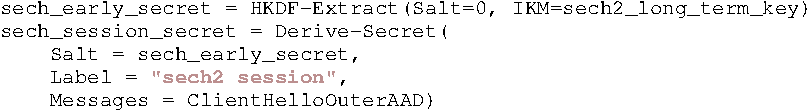
\includegraphics[width=\linewidth]{figure/sech2-derive-secret.pdf}
\captionsetup{width=.8\linewidth} 
\caption[SECH 2 Derive Secret]{Derive $sk_c$, the secret key that will be used by the client to encrypt $pt$ which has the inner \var{CH} data.}
\label{lst:sech2-derive-secret}
\end{listing}

The client encrypts $pt$ (authenticating $aad$) with $(\nonce,sk_c)$ using AES-128-GCM, producing a \sechtwotaglen{} octet authentication tag $t$ and the \sechtwocipherlen{} octet encrypted text $ct$. The \ac{CHO} has $c:=\nonce||ct||t$. The placement of the required values in cover $c$ of the \ac{CHO} is depicted in Figure~\ref{fig:sech2-cover}.
Finally the \ac{PSK} \var{binders} are inserted, which digest the \nonce, $ct$, and $t$.

\begin{figure}[htb]
\centering
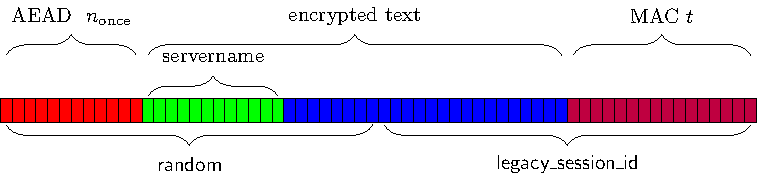
\includegraphics[width=\linewidth]{figure/sech2-cover.pdf}
\captionsetup{width=.8\linewidth} 
\caption[SECH 2 Cover]{Locations of AEAD inputs and outputs in the 64 octets of \ac{CH}\var{.random} and \ac{CH}\var{.legacy\_session\_id}. The cipher text $ct$ and MAC tag $t$ outputs are a function of $iv$, $sk_c$, $pt$, and $aad$: $(ct,t)=\text{AEAD}(iv,sk_c,pt,aad)$.}
\label{fig:sech2-cover}
\end{figure}

A cooperating server in possession of \varsechlongtermkey{} that receives a \ac{CH}
first constructs \var{ClientHelloOuterAAD}, then $sk_c$,
and attempts to decrypt and authenticate $ct$.
If decryption/authentication are unsuccessful the server continues with the \ac{TLS} 1.3 handshake as normal.
If successful, the client-facing server forwards \ac{CHI} to the backend server identified by the inner server name.
If the inner server name does not identify a backend server then the client-facing server continues the \ac{TLS} 1.3 handshake as if \ac{SECH} 2 is disabled.

The \ac{CHI} message  is a clone of \ac{CHO} but with:
1. the encrypted AEAD output $ct$ replaced with the plain text $pt$, as well as
2. the \var{extension\_data} field of the \var{server\_name} extension set to all 0s with the same length as the cover value for \var{server\_name} (The backend server does not learn the cover \ac{SNI} used).
The \ac{AEAD} \nonce and \ac{MAC} $t$ are left in \var{ClientHelloInner}.

The backend server can distinguish a \ac{CHI}
from a regular \ac{CH} by the \var{server\_name} extension.
If the \var{extension\_data} field of the \var{server\_name} has all 0s it is treated as a \var{ClientHelloInner}.
Otherwise it should be treated as a regular \ac{TLS} 1.3 \ac{CH}.
Note that if an attacker can send \ac{CH} directly to
the backend server,
then the client's reaction to an all zero \ac{SNI} can break
channel-level \ac{PC}.
For this reason the backend server must only process messages
from the client-facing server as \ac{CHI}s.
Authentication of the client-facing server is beyond the scope of this specification.
Also, a server tha receives a \ac{CH} whose \ac{SNI} is all 0s must abort with an appropriate alert. % TODO: how do clients typically react to an all zero \ac{SNI}

The server parses the plaintext $pt$
to retrieve the inner server name and inner \ac{ALPN} list
(if present)
in order to select an identity.
At this point the backend server might respond with \var{HRR} or \var{ServerHello}.
As discussed in Section~\ref{sec:hrr-hijacking} in the case of a \var{HRR}
the client and server essentially abandon the attempt to complete the \ac{SECH}
handshake successfully and craft the remaining messages solely for the purpose
of maintaining stealth.
This means the server should select an identity corresponding to the outer \ac{SNI}.
This can be achieved easily in shared-mode, but not split-mode,
since in split-mode the backend server for the outer \ac{SNI}
will not have seen the \ac{CH} or \ac{HRR} messages
needed for the transcript.
It is for this reason that our design of \ac{SECH} 2 does not work in split-mode.

%If the server accepts the first \ac{CHO}
%\ac{SECH} can proceed.
%Whereas in \ac{ECH} the acceptance signal is always sent in the server's first message
%(whether it is a \var{HRR} or \var{SH}),
%for \ac{SECH} 2 the acceptance signal is always in the \var{SH}.
%The client-facing server forwards these (and subsequent) messages to the client unaltered.
If the backend server accepts the parameters of \ac{CHI}
and accepts the inner servername identified in $pt$,
then it responds with a special \ac{SH} containing an \ac{SECH} acceptance signal.
Also, if using certificate-based authentication, then the later \ac{tlsC} message should contain a certificate identified by $pt$.

\begin{listing}[H]
\centering
\fbox{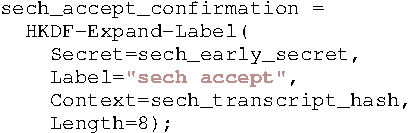
\includegraphics[width=.7\linewidth]{figure/sech2-accept-function.pdf}}
\captionsetup{width=.8\linewidth} 
\caption[SECH 2 Accept Confirmation]{The function used to calculate the SECH 2 acceptance signal using the \var{HKDF-Expand-Label} function defined in Section 7.1 of RFC 8446 (\cite{rfc8446}). The \var{sech\_early\_secret} is derived from $s$ as defined in Listing~\ref{lst:sech2-derive-secret}, and \var{sech\_transcript\_hash} is described in Listing~\ref{lst:sech2-transcript-hash}.}
\label{lst:sech2-accept-function}
\end{listing}

The \ac{SECH} 2 acceptance signal is 24 octets long and placed in the first 24 bytes of the \ac{SH}\var{.random},
such that it does not overlap with the \ac{ECH} acceptance signal.
It is a function of a hash of the transcript of the handshake so far, \varsechtranscripthash{},
and $s=$\varsechlongtermkey{}.
We define \varsechacceptconfirmation{} in Listing~\ref{lst:sech2-accept-function} and \varsechtranscripthash{} in Listing~\ref{lst:sech2-transcript-hash}.

\begin{listing}[H]
\centering
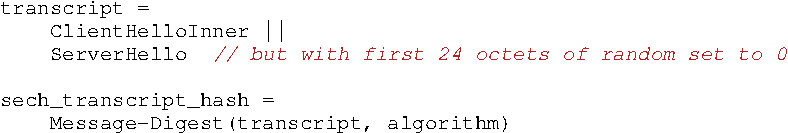
\includegraphics[width=\linewidth]{figure/sech2-transcript-hash.pdf}
\captionsetup{width=.8\linewidth} 
\caption[SECH 2 Transcript Hash]{Specification of the \var{sech\_transcript\_hash} used to calculate \var{sech\_accept\_confirmation}. The \var{algorithm} is the hash algorithm of the negotiated cipher suite for the handshake.}
\label{lst:sech2-transcript-hash}
\end{listing}

% The client uses that secret to encrypt the true target servername as well as a 32 byte secret inner nonce which are hidden in the ClientHello \var{random} and the \var{pre\_shared\_key} extension. The inclusion of the secret inner nonce is necessary to mitigate cut-and-paste attacks.

% More precisely, the client generates a 12 byte initialisation vector for AES-128-GCM. The plaintext is an ASCII encoding of the servername padded with 0x00 up to 12 bytes, appended to the 32 byte inner nonce.
% AEAD is used but the AAD is 0-length. % TODO: might be better to use the transcript hash of ClientHello (with random zeroed) as AAD, (however, if random is zeroed then transcript hash might not change)
% The AEAD tag is truncated to 8 bytes, such that we have a combined 64 bytes to send, which are put into the \var{ClientHello.random} and \var{ClientHello.legacy\_session\_id}. The first 12 bytes contain the IV, the next 12 contain the first 12 bytes of the cipher text, and the last 8 bytes of the \var{random} contain the truncated MAC, and the \var{ClientHello.legacy\_session\_id} is the last 

If the backend server accepts SECH 2 then it makes the SECH inner servername available to the application program via a callback or some other means, which allows the application program to decide whether or not to switch contexts (server certificate etc.).

%\subsubsection{SECH 2 with PSK}
%If a server accepts \ac{SECH} 2 it may issue a ticket referencing a \ac{PSK} that can be used to resume with backend server without stealthy encryption.

%The \ac{PSK} is derived as defined in Listing~\ref{lst:sech2-psk}, which differs from the definition of the PSK defined RFC 8446 in that the label is \var{``sech res''} rather than \var{``resumption''}. This ensures that the standard TLS 1.3 PSK is only used for a connection to the outer servername, whereas the \var{sech2\_psk} is only used for the inner servername.
%\begin{listing}
%\begin{verbatim}
%sech2_psk = HKDF-Expand-Label(
%    resumption_master_secret,
%    "sech res",
%    ticket_nonce,
%    Hash.length)
%\end{verbatim}
%\caption{\label{lst:sech2-psk}Definition of the PSK used when resuming an SECH 2 session.}
%\end{listing}

%Note that this definition of \var{sech2\_psk} is a function of the \var{resumption\_master\_secret}, which is not available to a client-facing server in split-mode.
%Therefore, this type of resumption is not possible in split-mode. % TODO: design PSK resumption for split mode
% TODO: what if sech2_psk and psk are the same, e.g. because they collide when using different ticket_nonces? maybe the label should still be "sech res" but each ticket_nonce should be marked as either sech or non-sech?

\subsection{Distributing SECH 2 access without sharing \var{sech2\-\_long\-\_term\_secret}}

To use a resumption \ac{PSK} (sent via \var{NewSessionTicket}) in TLS 1.3 the PSK
is bound cryptographically to the transcript of the first handshake as well as most of the \var{CH} for the second handshake.
The binding to the first handshake arises because the \ac{PSK} is derived from the key schedule
of the first handshake.
The binding to the second handshake is achieved using the \var{binder} value.
Pseudo-code for the construction of the \var{binder} value is presented in Listing~\ref{lst:binder-pseudocode}.

\begin{listing}
    \begin{verbatim}
early_secret = HKDF-Extract(0, PSK)
binder_key = Derive-Secret(early_secret, "res binder", "")
binder_finished_key = HKDF-Expand-Label(
    binder_key,
    "finished",
    "",
    Hash.length)
binder =
    HMAC(binder_finished_key,
        Transcript-Hash(ClientHello))
    \end{verbatim}
    \captionsetup{width=.8\linewidth} 
    \caption[Pseudo-code for Computation of  \var{binder}]{\label{lst:binder-pseudocode}Pseudo-code of the process used to compute a \var{binder} when using a resumption PSK. The \var{HandshakeContext1} is the transcript of the handshake in which the PSK was derived, and \var{ClientHello} is for a new connection and is truncated so as not to include the \var{binders} list itself. This formulation is tweaked slightly in the case of SECH 2.}
\end{listing}


% [ ] TODO research has anyone done ticket sharing amongst clients before? E.g. client with multiple processes

% [ ] TODO bleichenbacher attack

Sharing the SECH 2 long term secret widely amongst clients would violate the `Avoid Widely Shared Secrets' requirement advocated by \citep{rfc8744-issues}. How do we facilitate connections from large numbers of clients while restricting each long term secret to being shared to only 2 parties? One option is to have a distinct long term secret for each client-server pair. The SECH 2 design specified here can facilitate this through trial decryption, i.e. every \var{ClientHello} processed by the server is checked against each registered secret until one is found to successfully decrypt the inner server name. This approach scales horribly, with the cost of every connection being proportional to the number of registered clients, whether or not those clients are active. But note that this trial decryption process is highly parallelizable.

Our approach to distributing access to the \ac{SECH} 2 capability
exploits \ac{PSK}s, either via gossiping or bootstrapping.
The first step is for a client C1 to establish a resumption \ac{PSK} with
the client-facing server.
For the bootstrap approach: in a subsequent connection the client can use this \ac{PSK}
as if it were the \var{sech2\_long\_term\_key}, while also supplying
the \ac{PSK} identity in the \ac{PSK} extension.
Similarly for the gossiping approach C1 passes the \ac{PSK} (and associated identity)
to another client C2, and C2 uses this \ac{PSK} to perform \ac{SECH} 2.
The backend server will not recognise the \ac{PSK} identity and ignores it.

In split-mode, the initial bootstrap connection is with the client-facing server, whereas
the \ac{SECH} 2 conneciton is with the backend server. This means the second connection
cannot itself be used to establish \ac{PSK}s for subsequent connections.
The bootstrap connection yields some number $n$ of \ac{PSK}s that can be used for connecting
to the backend server, but once these \ac{PSK}s are expended the bootstrap step has to be repeated.

%\begin{listing}
%    \begin{verbatim}
%binder =
%    HMAC(binder_key,
%        Transcript-Hash(ClientHello))
%    \end{verbatim}
%    \captionsetup{width=.8\linewidth} 
%    \caption{\label{lst:binder-sech2-pseudocode-ext}Calculation of \var{binder} for SECH 2 bootstrap \acp{PSK}.}
%\end{listing}

%[ ] The server uses the 32 byte shared secret key as well as the decrypted inner servername to create an 8 byte acceptance signal which is hidden in the ServerHello.random. The 8 byte acceptance signal is computed as \var{sech\_accept\_confirmation = AEAD-encrypt(IV, plaintext="", aad=sech\_inner\_servername, accept\_key).tag}, where IV is the first 12 bytes of the ServerHello.random (uniformly randomly generated), the plaintext is zero-length, the AAD is precisely the inner servername (which does not need to be transmitted because it is known by the client), and \var{accept\_key} is a session-specific key derived using HKDF from the session's master secret and the transcript of ClientHello..ServerHello, but with the last 16 bytes of ServerHello.random set to 0x00. The last 8 bytes of \var{ServerHello.random} are possibly used for an ECH acceptance signal, and the ECH acceptance signal is computed based on the transcript of ClientHello..ServerHello, except with the last 8 bytes of of ServerHello.random set to 0x00. Therefore, if the server is sending an SECH acceptance signal *and* an ECH acceptance signal, the SECH acceptance signal is computed first because the ECH acceptance signal is defined to incorporate the SECH acceptance signal bytes in its transcript hash. To construct the 8 sech\_accept\_confirmation bytes we make use of the HKDF-Expand-Label function defined in RFC 8446 Section 7.1.
    % ```c
    % md = TranscriptHash(ClientHello..ServerHello) // with last 16 bytes of ServerHello.random set to 0x00
    % padded\_sech\_IV = pad(sech\_IV, HashLen)
    % sech\_accept\_confirmation = HKDF-Expand-Label(
    %   HKDF-Extract(padded\_sech\_IV, sech\_symmetric\_key),
    %   "sech ac" || 0x00 || sech\_decrypted\_inner\_servername,
    %   md,
    %   8
    % )
    % ```

\subsection{Design Differences Between SECH 2 and ECH}
[ ] The acceptance signal is always sent in the \var{ServerHello}

[ ] This definition of \var{sech\_accept\_confirmation} is essentially a modification of the ECH \var{accept\_confirmation} defined in Section 7.2 of [TODO cite ECH draft], which we repeat here:
% ```
%   accept\_confirmation = HKDF-Expand-Label(
%     HKDF-Extract(0, ClientHelloInner.random),
%     "ech accept confirmation",
%     transcript\_ech\_conf,
%     8
%   )
% ```

The ECH \var{accept\_confirmation} uses \var{HKDF-Extract(0, ClientHelloInner.random)} as the `Secret' passed to \var{HKDF-Expand-Label}, and \var{HKDF-Extract(0,ClientHelloInner.random)} is confidential (only known to the client and server) because the \var{ClientHelloInner.random} was in the {\em encrypted} \var{ClientHelloInner}. Also, it is essential that \var{accept\_confirmation} can be generated by the backend server in ECH split mode, which is why the salt passed to \var{HKDF-Extract} is the 0 string. While it would be more secure to use a session-specific random value as the salt for \var{HKDF-Extract}, we cannot use the \var{ClientHelloOuter.random} because this value is not available to the backend server (the backend server only processes the ClientHelloInner). The HKDF specification assumes that the salt and IKM passed to HKDF-Extract are indepedent of each other (Section 3.4 RFC 5869), and in particular that the salt values are not `chosen or manipulated by an attacker'.
Since \var{ClientHelloOuter.random} is never processed by the backend server it will not be incorporated into the \var{Finished} message, which means it is not protected from tampering in split-mode. This means an attacker could manipulate \var{ClientHelloOuter.random} and so it should not be used as the salt for \var{HKDF-Extract}.

[ ] In order to facilitate a split mode of operation in a similar fashion to ECH it must be possible for the SECH backend server to produce  the \var{sech\_accept\_confirmation} signal. For the signal described above this entails that the backend server must possess the \var{sech\_symmetric\_key}, meaning \var{sech\_symmetric\_key} would be shared amongst three parties; client, client-facing server, backend server. This violates one of the design requirements listed in Section 3.2 by \cite{rfc8744-issues}; Avoid Widely Shared Secrets.
% \subsection{Security Considerations}

[ ] High probability for situations where an attacker can guess the plaintext, or where there are only a small number of possible plaintexts (SNIs). How does this affect capacity to brute force the secret key? -> Does this mean the SNIs must also remain secret?

\subsection{Implementation Notes}
I have implemented the above \ac{SECH} 2 design in a fork of OpenSSL codebase.
[ ] Error handling
\subsection{Testing}

I have implemented the following basic tests of the \ac{SECH} 2 implementation and \ac{API} using the OpenSSL test infrastructure. Writing tests in this way has the advantage of comfortably allowing granular tests for specific errors and conditions at specific points of execution. A disadvantage is that the tests I have written involving a client and server do not actually use the system's network and hence cannot be easily inspected with external tools like Wireshark.

The \var{test\_sech2\_roundtrip\_accept\_and\_resume\_with\_ticket} first performs the same test as \var{test\_sech2\_roundtrip\_accept} but then additionally tests that the client can reconnect to the server using a resumption \ac{PSK} derived from the first connection. This test revealed an interesting bug and design flaw during development. In an earlier design the \ac{SECH} 2 session key was derived from a transcript of the full \var{ClientHello} including the \var{pre\_shared\_key} extension. However, the \var{binder} values in the \var{pre\_shared\_key} extension are also bound to the rest of \var{ClientHello}. If the session key is bound to the \var{binder} and then used to edit an earlier part of the \var{ClientHello} then the \var{binder} is invalidated. The solution is that the session key should be derived from the \var{ClientHello} up to but not including the \var{binder}, and the \ac{SECH} 2 encryption has to take place before the \var{binder} is calculated.
\section{SECH 5}
\subsection{Motivations and Deployment Scenarios}

[ ] arbitrary access for new clients without coordination from server

\subsection{Design}

A server produces an \var{SECHConfig} which specifies a \ac{HPKE} cipher suite
(\ac{KEM}, \ac{HKDF}, and \ac{AEAD} IDs),
a public key for the \ac{KEM}, and the server
also maintains the corresponding private key for the public key.
For simplicity in this specification we assert that the \ac{HKDF}
and \ac{AEAD} are chosen at \var{SECHConfig}-compilation time.
This is unlike \ac{ECH} where the \ac{HKDF} and \ac{AEAD} are
negotiated for each session.

A client has to securely obtain the \var{SECHConfig} in order to offer \ac{SECH} 5 in a \var{ClientHello}, e.g. using \ac{DoH} or by any other secure and confidential means.

The client first produces the \var{ClientHello} as would be done normally
for \ac{TLS} 1.3 up to the point of computing the \ac{PSK} \var{binder}.

The client instantiates a \ac{HPKE} context using the suite specified in
the \var{SECHConfig} and produces a 32 octet \var{enc}.
As of writing the only \ac{KEM} with a 32 octet \var{enc} in the \ac{IANA} is
the \ac{X25519} \ac{EC}.
The \var{enc} is produced by generating a 32 octet random key, $k$, and then encrypting
that key with the public key from the \var{SECHConfig}.
The \var{random} field is set to value of \var{enc}.

The client concatenates the inner servername and inner \ac{ALPN} list separated by null bytes, and pads this to 16 bytes with 0s. Call the resulting string \var{sech\_cleartext}.
The client creates \var{ClientHelloOuterAAD} which is a clone
of the \var{ClientHello} but with the \var{legacy\-\_session\-\_id} field set to 0s,
and the \var{binders} list truncated off.
Using the \ac{AEAD} specified in the \var{SECHConfig} the client encrypts
\var{sech\_cleartext} with \var{ClientHelloOuterADD} as \ac{AAD}
producing a 32 octet ciphertext \var{sech\_cipher}
(including the 16 byte \ac{AEAD} tag). 
For simplicity we assert in this draft that only \ac{AEAD}s with a 16 byte tag are valid in an \var{SECHConfig}.

% [ ] client encrypts the \var{padded\_servername} with the AEAD specified in SECHConfig, and with key $k$ and a \nonce which is the first 12 octets of the hash of \var{SECH5ClientHelloAAD}, and with \var{SECH5ClientHelloAAD} as AAD, producing \var{sech5\_cipher} which is the concatenation of the encrypted text and the tag $t$

% [ ] \var{SECH5ClientHelloAAD} is the \var{ClientHello} but with the portion in which the AEAD cipher (encrypted text and tag) will be placed set to zero, the size and location of this region depends on \var{SECHConfig}

% [ ] \var{SECH5ClientHelloAAD} is the \var{ClientHelloOuter} but with the \var{random} and \var{legacy\_session\_id} set to all 0s

The client encodes \var{enc} and \var{sech\_cipher} in the \var{ClientHello} \var{random} and \var{legacy\_session\_id} fields producing a partial \var{ClientHelloOuter}
(excluding the \var{binders})
as depicted in Figure~\ref{fig:sech5-cover}.
If the client is using a resumption \ac{PSK} controlled by the backend server
the \var{binders} list is computed
using the synthetic \var{ClientHelloInner} transcript rather
than the transcript of \var{ClientHelloOuter}.

The \var{ClientHelloInner} has the \var{random} field replaced with \varsechinnerrandom{}, and the first 16 bytes of the
\varlegacysessionid{} replaced with \var{sech\_clear}.
Also, the extension data field of the outer \ac{SNI} is set to all 0s.

The client-facing server attempts to decapsulate \var{enc} with the private key associated with \var{SECHConfig} retrieving $k$, on failure 
the client-facing server continues with normal TLS 1.3,
although implementations should ensure that the timing of the response in case of \ac{SECH}
decryption failure is not distinguishable from the case when
\ac{SECH} succeeds.
Using the \ac{HKDF} in \var{SECHConfig} $k$ is transformed into \varsechinnerrandom{}.

% [ ] TODO: Unlike \ac{ECH} we do not support arbitrary numbers \var{SECHConfig}s on the server
% in order to ensure the server response time is consistent and does not reveal \ac{SECH}
% decryption success or failure. 

The client-facing server computes \var{ClientHelloOuterAAD} and the \nonce, and then attempts to decrypt and retrieve \var{sech\_cleartext}, on failure  
the client-facing server continues with a normal TLS 1.3 handshake.

On success the client-facing server constructs \var{ClientHelloInner} by replacing 
the first 16 bytes of \var{ClientHelloOuter}'s \var{legacy\-\_session\-\_id}
with \var{sech\_clear}, and also replacing the \var{random} field
with $k$. Also the \var{extension\_data} of the \var{server\_name} extension is set to all 0s.

The client-facing server forwards \var{ClientHelloInner} to the backend server
(over a channel secured and authenticated by some other means).
The backend server processes this message, detecting the all-zero \ac{SNI} extension value,
and decodes the inner \ac{SNI} and \ac{ALPN} from the \varlegacysessionid{}.

If the backend server needs to negotiate different parameters by sending a
\var{HelloRetryRequest} this message is constructed as in normal \ac{TLS} 1.3.
The \var{HelloRetryRequest} message has no cover for a stealthy acceptance signal.

The subsequent \var{ClientHello2}'s \var{random} and \varlegacysessionid{} fields
must be identical to the first \var{ClientHello} so as not to stick out from normal
\ac{TLS} 1.3. This means the \var{ClientHello2} has no cover for hiding a second
\ac{SECH} payload, which means the \var{ClientHello2} is malleable and 
vulnerable to \var{HelloRetryRequest} hijacking.
Therefore, in the case of a \var{HRR} the remainder of the handshake is simply intended
to prevent revelation to the attacker that \ac{SECH} was attempted, and
the client and backend server give up on the connection.

To achieve this, when a client-facing server receives a \var{ClientHello2} it always
forwards it to the backend server corresponding to the outer \ac{SNI} in the \var{ClientHello2}. Ideally this `cover' backend server should support a superset of
the parameters supported by all \ac{SECH} backend servers such that the \var{ClientHello2}
will be accepted by the `cover' backend.

In the case that no \var{HRR} is triggered the backend server can continue to signal
its acceptance of \ac{SECH}.
The \var{ServerHello} contains a special \var{sech\_accept\_confirmation} value in the last 8 octets of the \var{random} field.


\begin{figure}[htb]
\centering
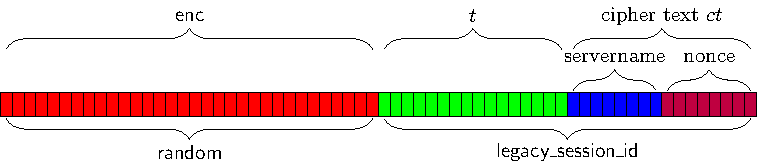
\includegraphics[width=\linewidth]{figure/sech5-cover.pdf}
\captionsetup{width=.8\linewidth} 
\caption[SECH 5 Cover]{}
\label{fig:sech5-cover}
\end{figure}

\subsection{Implementation Notes}